\section{Моделирование предметной области}
\label{sec:model}

\subsection{Модель социальных сил в моделировании пешеходных потоков}
\label{sec:model:sf}

В данном разделе будет более подробно рассмотрена оригинальная модель социальных сил, описанная в работе Дирка Хелбинга~\cite{helbing_social_force}.

Также в данном разделе предложены модификации модели социальных и рассмотрены дополнительные социальные силы, используемые в разрабатываемом ПС.

\subsubsection{Общее описание модели социальных сил}
\label{sec:model:sf:description}

Основной концепцией в модели социальных сил является абстрактное понятие социальной силы.
Под социальной силой понимается мера мотивации пешехода двигаться в определенном направлении.
Таким образом, социальная сила представляет собой направленный вектор.
Итоговое направление и некоторая мера скорости движения определяется как векторная сумма всех социальных сил, воздействующих на человека.

В модели социальных сил рассматривается две социальных силы, без которых модель не была бы корректной: движущая сила и сила отталкивания.
Движущая сила более подробно рассмотрена в разделе~\ref{sec:model:sf:moving_force}, а отталкивающая сила "--- в разделе~\ref{sec:model:sf:repulsion_force}.

Важным моментом является учет поля зрения пешехода. В разделе~\ref{sec:model:sf:fov} описано как оригинальное решение авторов модели, так и решение, используемое в разрабатываемом ПС.

Также стоит упомянуть о концепции флуктуаций, которая описана в разделе~\ref{sec:model:sf:fluctuation}.

% Последним вопросом, рассматриваемым в разделе~\ref{sec:model:sf:panic}, является моделирование паники с помощью модели социальных сил.

Наглядное описание всех используемых в проекте социальных сил представлено на рисунке~\ref{sec:model:sf:social_forces_pic}.

\begin{figure}[!ht]
  \centering
  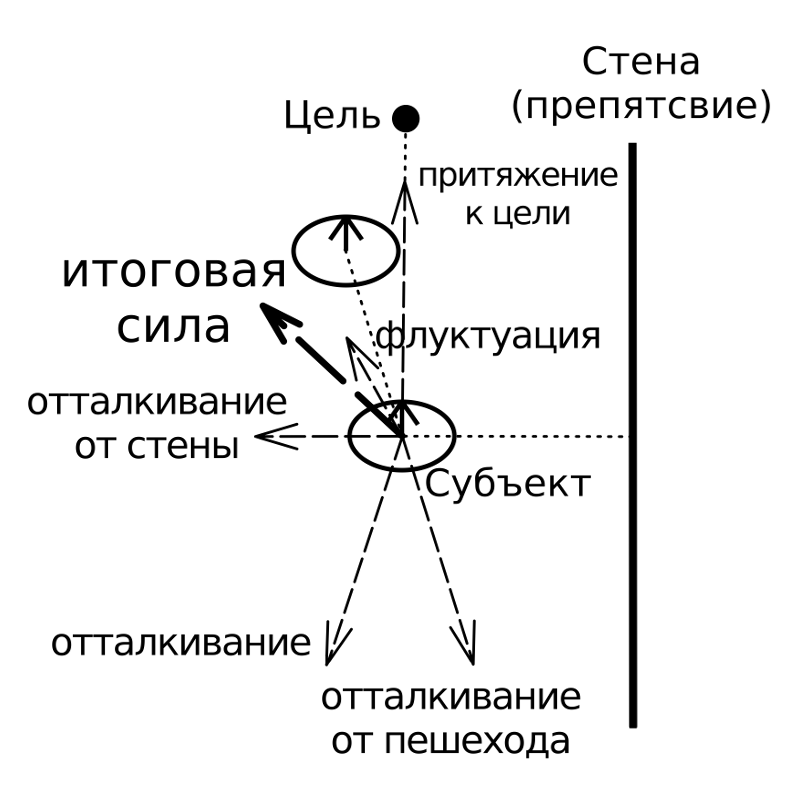
\includegraphics[width=\linewidth]{social_forces}
  \caption{Используемые социальные силы}
  \label{sec:model:sf:social_forces_pic}
\end{figure}

\subsubsection{Движущая сила в модели социальных сил}
\label{sec:model:sf:moving_force}

Движущая сила представляет побуждение пешехода достичь своей цели.
В случае, если цель не находится в прямой видимости, вводится последовательность промежуточных целей $\vec{r}_\alpha^k$.

Для полного описания движущей силы введем понятия желаемого направления и желаемой скорости.

Желаемое направление "--- вектор направления к следующей промежуточной цели, который определяется как:
\begin{equation}
  \label{sec:model:sf:moving_force:desired_direction_fm}
  \vec{e}_\alpha(t) = \vec{r}_\alpha^k - \vec{r}_\alpha(t)
\end{equation}
\begin{explanation}
где & $ \vec{r}_\alpha^k $ & вектор следующей промежуточной цели пешехода $\alpha$; \\
    & $ \vec{r}_\alpha(t) $ & текущая позиция пешехода $\alpha$ в момент времени $t$.
\end{explanation}

Желаемая скорость "--- скорость, с которой пешеход предпочел бы двигаться к цели.
В модели сделано предположение, что желаемая скорость пешеходов распределена нормально со средним значением в $1.34$ м/с и среднеквадратичным отклонением в $0.26$ м/с.

Также в оригинальной модели был введен вектор желаемой скорости $\vec{v}_\alpha^0(t)$
\begin{equation}
  \label{sec:model:sf:moving_force:desired_speed_fm}
  \vec{v}_\alpha^0(t) = v_\alpha^0(t) \vec{e}_\alpha(t)
\end{equation}
\begin{explanation}
где & $ v_\alpha^0 $ & желаемая скорость пешехода $\alpha$.
\end{explanation}

И выполнялась коррекция текущего направления движения с учетом времени релаксации (примерно $0.5$ с).
\begin{equation}
  \label{sec:model:sf:moving_force:force_fm}
  \vec{F}_\alpha^{moving}(t) = {{1}\over{t_\alpha}} ( \vec{v}_\alpha^0(t) - \vec{v}_\alpha(t) )
\end{equation}
\begin{explanation}
где & $ t_\alpha $ & время релаксации пешехода $\alpha$; \\
    & $ \vec{v}_\alpha(t) $ & текущая скорость пешехода $\alpha$ в момент времени $t$.
\end{explanation}

Таким образом, в оригинальной модели пешеход двигался не с желаемой скоростью в выбранном направлении, а с желаемой скоростью по направлению к цели.
В случае отсутствия каких-либо других социальных сил данное различие несущественно, однако оно может сильно исказить результаты при наличии социальных сил,
  имеющих схожее с движущей силой происхождение (например, при наличии силы объединения пешеходов в группы).

В связи с этим было принято решение выполнять коррекцию желаемой скорости не по одной движущей силе, а по сумме всех воздействующих сил.
Этим обеспечивается поддержание желаемой скорости вне зависимости от текущего направления движения.

\subsubsection{Отталкивающая сила в модели социальных сил}
\label{sec:model:sf:repulsion_force}

Сила отталкивания представляет побуждение пешехода сохранять некоторую дистанцию до других пешеходов и препятствий (стен).
Она направлена в противоположную от ближайшей точки препятствия сторону, а ее модуль в общем случае обратно зависит от расстояния до препятствия.
Авторы оригинальной модели социальных сил предлагают ввести поправочный коэффициент для учета анизотропности данной силы: пешеход держит большую дистанцию спереди и сзади, и меньшую – с боков.
Таким образом, модуль данной силы зависит не только от расстояния, но еще и от направления.

Отталкивающая сила между пешеходом $\alpha$ и препятсвием $\beta$ выражается как:
\begin{equation}
  \label{sec:model:sf:repulsion_force:force_fm}
  \vec{F}_{\alpha\beta}^{repulsion}(\vec{r}_{\alpha\beta}) = - \nabla V(r_{\alpha\beta})
\end{equation}
\begin{explanation}
где & $ r_{\alpha\beta} = r_\alpha - r_\beta $ & вектор направления от $\alpha$ к ближайшей точке $\beta$; \\
    & $ V(r_{\alpha\beta}) $ & функция, эквипотенциальные линии которой имеют форму эллипса.
\end{explanation}

\subsubsection{Учет поля зрения пешехода в модели социальных сил}
\label{sec:model:sf:fov}

Для большинства социальных сил имеет значение, мог ли данный пешеход видеть источник данной силы.
Для решения данной проблемы авторы оригинальной модели ввели еще один коэффициент, зависящий от угла между направлением движения и источником силы.
Данный коэффициент равен $1$, если угол между направлением движения и источником силы по модулю меньше некоторого заданного значения (в работе использовалось значение $100$ градусов), или $0.5$ в обратном случае.

Очевидным улучшением предложенной модели будет использование не дискретного порога, а некоторой непрерывной функции.

Для наглядности эту функцию можно представлять в виде некоторой формы на двумерной плоскости.
Интуитивно понятно, что данная форма представляет собой форму поля зрения пешехода.
Значение весовой функции определяется как длина вектора от центра координат к точке пересечения луча, проведенного из начала координат под соответствующим углом.

\begin{figure}[ht]
\centering
  \begin{subfigure}[b]{0.45\textwidth}
    \centering
    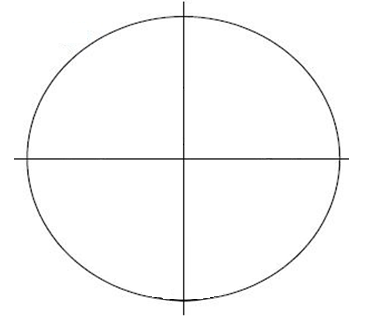
\includegraphics[scale=0.4]{fov_isotropic.png}
    \caption{}
  \end{subfigure}
  \begin{subfigure}[b]{0.45\textwidth}
    \centering
    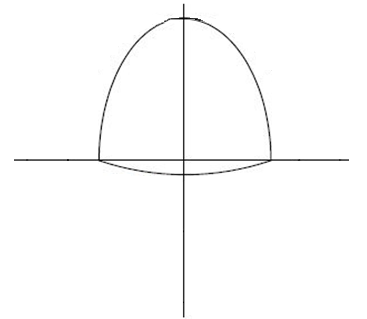
\includegraphics[scale=0.4]{fov_anisotropic.png}
    \caption{}
  \end{subfigure}
  \caption{ Примеры форм поля зрения пешехода: а "--- изотропная форма зрения;
            б "--- анизотропная форма зрения}
  \label{sec:model:sf:fov:example_figure}
\end{figure}

\subsubsection{Флуктуации в модели социальных сил}
\label{sec:model:sf:fluctuation}

Для более реалистичного поведения к итоговой сумме всех сил добавляются некоторые случайные флуктуации.
Основой флуктуаций с социальной точки зрения являются неучтенные мотивации или случайные импульсные решения пешехода.

Также добавление флуктуаций позволяет выходить из «тупиковых» ситуаций, когда сумма всех сил близка по модулю к нулю.

% не реализовано в ПС
\begin{comment}
\subsubsection{Моделирование паники с использованием модели социальных сил}
\label{sec:model:sf:panic}

Важным сценарием при тестировании является сценарий паники. В данном случае поведение пешеходных потоков значительно меняется и требует других средств и методов моделирования.

На основе изучения различных социальных исследований, выделяют следующие отличия в поведении людей при панике \cite{helbing_panic}:
\begin{itemize}
  \item люди двигаются (или пытаются двигаться) значительно быстрее чем обычно;
  \item люди перестают поддерживать безопасное личное расстояние и начинают взаимодействовать физически;
  \item люди начинают проявлять склонность к массовому поведению (повторять поведение окружающих людей).
\end{itemize}

Для того, чтобы учесть данные отличия, введем в модель некоторые переменные.

Первой переменной, необходимой для моделирования сценария паники, является уровень паники.
Источниками паники являются какие-либо опасные объекты.
Также уровень паники может распространятся по близко стоящим друг к другу людям.
Определим уровень паники как
\begin{equation}
  \label{sec:model:sf:panic:level}
  ppl_\alpha = kspl \sum\limits_{i=1}^n {{ppl_i}\over{||\vec{r}_\alpha - \vec{r}_i||}} + kdpl \sum\limits_{i=1}^m {{spl_i}\over{||\vec{r}_\alpha - \vec{r}_i||}}
\end{equation}
\begin{explanation}
где & $ kspl $ & коэффициент распространения паники; \\
    & $ kdpl $ & коэффициент начального приобретения паники; \\
    & $ ppl_i $ & уровень паники $i$-ого пешехода; \\
    & $ spl_i $ & уровень паники $i$-ого опасного объекта; \\
    & $ n $ & количество других пешеходов в поле зрения пешехода; \\
    & $ m $ & количество опасных объектов в поле зрения пешехода; \\
    & $ ||\vec{r}_\alpha - \vec{r}_i|| $ & расстояние от пешехода $\alpha$ до источника паники $i$.
\end{explanation}

Также следует отметить важность выбора коэффициента распространения паники $kspl$.
Если установить для данного значения слишком низкое значение, то эффект лавинообразного возникновения паники не появится.
Если же установить слишком высокое значение, то пешеходы могут войти в состояние паники даже от незначительных воздействий.

Желаемая скорость с учетом паники определяется как

\begin{equation}
  \label{sec:model:sf:panic:desired_speed}
  vpanic_\alpha^0 = kspeedpl \cdot ppl_\alpha v_\alpha^0
\end{equation}
\begin{explanation}
где & $ kspeedpl $ & коэффициент учета паники в желаемой скорости.
\end{explanation}

А отталкивающая сила определяется как

\begin{equation}
  \label{sec:model:sf:panic:repulsion_force}
  \vec{Fpanic}_{\alpha\beta}^{repulsion}(\vec{r}_{\alpha\beta}) = krepulsionpl {{1}\over{ppl_\alpha ppl_\beta}}\vec{F}_{\alpha\beta}^{repulsion}(\vec{r}_{\alpha\beta})
\end{equation}
\begin{explanation}
где & $ kspeedpl $ & коэффициент учета паники в силе отталкивания.
\end{explanation}

Также люди начинают копировать желаемое направление окружающих людей. Этот эффект можно описать как

\begin{equation}
  \label{sec:model:sf:moving_force:desired_direction_fm}
  \vec{epanic}_\alpha(t) = kdirectionpl \cdot ppl_\alpha \sum\limits_{i=1}^n \vec{e}_\alpha(t)
\end{equation}
\begin{explanation}
где & $ kdirectionpl $ & коэффициент учета паники в желаемом направлении; \\
    & $ n $ & количество других пешеходов в поле зрения пешехода.
\end{explanation}

\subsection{Функциональная спецификация разрабатываемого ПС}
\label{sec:model:func_spec}

В результате анализа предметной области и разработки собственной модификации модели социальных сил, к разрабатываемому ПС были выдвинуты следующие функциональные требования:
\begin{itemize}
  \item Разрабатываемое ПС должно выполнять симуляцию пещеходных потоков по модели социальных сил.
        Входными данными являются сценарий симуляции и план помещения, а выходными "--- либо файл с результатами моделирования в унифицированном формате, либо 2D анимация с отмеченными вероятными местами скопления людей.
        План помещения задается в формате SVG, где значимым с точки зрения симуляции объектам проставлены определенные атрибуты.
        Все используемые форматы (формат сценария симуляции, формат результатов моделирования, формат плана помещения) должны быть полностью описаны в документации.
  \item Разрабатываемое ПС должно позволять выполнять как симуляцию в режиме реального времени, так и воспроизведение заранее сгенерированного файла результатов симуляции.
  \item Гибкая настройка модели и сценария симуляции.
        Большинство значимых параметров модели и сценария должны быть изменяемыми из файла описания сценария симуляции.
  \item Наличие возможности интеграции моделирования в существующее приложение.
        Сторонние приложения могут импортировать результаты симуляции и выполнять над ними определенные действия.
  \item Высокая скорость работы.
        Разрабатываемое приложение должно обеспечивать возможность просмотра результатов симуляции в режиме реального времени для как минимум одной сотни пешеходов.
\end{itemize}
\end{comment}
